\documentclass[11pt,aspectratio=169]{beamer}

\usetheme{Madrid}
\usecolortheme{whale}
\setbeamertemplate{navigation symbols}{}
\setbeamertemplate{footline}{%
  \leavevmode\hbox{%
    \begin{beamercolorbox}[wd=.33\paperwidth,ht=2.5ex,dp=1ex,center]{author in head/foot}%
      \usebeamerfont{author in head/foot}\insertshortauthor
    \end{beamercolorbox}%
    \begin{beamercolorbox}[wd=.34\paperwidth,ht=2.5ex,dp=1ex,center]{title in head/foot}%
      \usebeamerfont{title in head/foot}\insertshorttitle
    \end{beamercolorbox}%
    \begin{beamercolorbox}[wd=.33\paperwidth,ht=2.5ex,dp=1ex,right]{date in head/foot}%
      \usebeamerfont{date in head/foot}\insertframenumber{} / \inserttotalframenumber\hspace*{2ex}
    \end{beamercolorbox}%
  }\vskip0pt%
}

\usepackage[T1]{fontenc}
\usepackage[utf8]{inputenc}
\usepackage{amsmath,amssymb}
\usepackage{booktabs}
\usepackage{graphicx}
\usepackage{xcolor}
\usepackage{array}

\graphicspath{{../figures/}}

\definecolor{accentblue}{HTML}{2471A3}
\definecolor{accentred}{HTML}{C0392B}
\definecolor{accentgreen}{HTML}{27AE60}
\definecolor{lightgray}{HTML}{F2F3F4}

\setbeamercolor{block title}{bg=accentblue,fg=white}
\setbeamercolor{block body}{bg=lightgray,fg=black}

\title[Math4AI Capstone]{From Linear Scores to a Single Hidden Layer}
\subtitle{A Mathematical Study of Simple Learning Systems}
\author[Feyzullayev, Samadov, Abdullazade]{Sharaf Feyzullayev \and Nicat Samadov \and Samir Abdullazade}
\institute{National AI Center --- AI Academy}
\date{Math4AI Final Capstone, March 2026}

\begin{document}

% ──────────────────────────────────────────
% SLIDE 1: Title
% ──────────────────────────────────────────
\begin{frame}
\titlepage
\end{frame}

% ──────────────────────────────────────────
% SLIDE 2: Central Question
% ──────────────────────────────────────────
\begin{frame}{The Central Question}

\begin{block}{Research Question}
\textit{When does a one-hidden-layer nonlinear classifier genuinely improve on a linear decision rule, and when is additional model complexity unnecessary?}
\end{block}

\vspace{0.6em}

\textbf{Our approach --- argue from evidence, not preference:}
\begin{itemize}
    \item Compare \textbf{softmax regression} (linear baseline) against a \textbf{one-hidden-layer neural network} ($\tanh$ + softmax)
    \item Three datasets of increasing geometric complexity: Gaussian blobs, moons, digits
    \item Derive the mathematics that each model relies on, then test experimentally
    \item \textbf{More complexity is not automatically better} --- if the linear baseline is sufficient, we say so and justify it
\end{itemize}

\vspace{0.3em}
\centering
\small\textcolor{accentblue}{\textbf{Everything implemented from scratch in NumPy --- no autograd, no PyTorch, no scikit-learn}}

\end{frame}

% ──────────────────────────────────────────
% SLIDE 2b: Fair Comparison
% ──────────────────────────────────────────
\begin{frame}{Why the Comparison is Fair}

Both models are evaluated under \textbf{identical conditions} to ensure a fair comparison:

\vspace{0.5em}
\begin{columns}[T]
\begin{column}{0.48\textwidth}
\textbf{Shared across models:}
\begin{itemize}
    \item Same train/val/test splits
    \item Same preprocessing (no extra transforms)
    \item Same $L_2$ regularisation ($\lambda = 10^{-4}$)
    \item Same epoch budget (200)
    \item Same mini-batch size (64)
    \item Same reporting metrics (accuracy + CE)
\end{itemize}
\end{column}
\begin{column}{0.48\textwidth}
\textbf{Model selection protocol:}
\begin{itemize}
    \item Best checkpoint chosen on \textbf{validation CE only}
    \item Test set touched \textbf{exactly once} per seed
    \item 5 random seeds with 95\% CI reporting
    \item[$\Rightarrow$] No cherry-picking, no test-set leakage
\end{itemize}

\vspace{0.4em}
\textbf{Key principle:}\\
The NN must \textit{earn} its complexity through evidence --- the linear baseline is the default.
\end{column}
\end{columns}

\end{frame}

% ──────────────────────────────────────────
% SLIDE 3: Models
% ──────────────────────────────────────────
\begin{frame}{Two Models, Same Objective}

\begin{columns}[T]
\begin{column}{0.48\textwidth}
\textbf{Model 1: Softmax Regression}
\[
s(x) = Wx + b
\]
\[
p_j(x) = \frac{\exp(s_j)}{\sum_\ell \exp(s_\ell)}
\]
\begin{itemize}
    \item \textbf{Geometry:} hyperplane boundaries
    \item 650 params on Digits ($Kd + K$)
    \item Represents exactly the family of affine classifiers
\end{itemize}
\end{column}

\begin{column}{0.48\textwidth}
\textbf{Model 2: One-Hidden-Layer NN}
\[
h = \tanh(W_1 x + b_1)
\]
\[
s = W_2 h + b_2
\]
\begin{itemize}
    \item \textbf{Geometry:} curved boundaries
    \item 2{,}410 params on Digits ($3.7\times$ more)
    \item Hidden layer = learned nonlinear coordinate change
\end{itemize}
\end{column}
\end{columns}

\vspace{0.5em}
\centering
Both minimise cross-entropy: $\;\mathcal{L} = -\frac{1}{n}\sum_i \log p_{y_i}(x_i)\;$ which \textbf{is} the negative log-likelihood under a categorical model

\end{frame}

% ──────────────────────────────────────────
% SLIDE 4: Backpropagation
% ──────────────────────────────────────────
\begin{frame}{Backpropagation: Chain Rule in Action}

\textbf{Idea:} propagate loss sensitivities backward through the computation graph.

\vspace{0.3em}
\begin{columns}[T]
\begin{column}{0.55\textwidth}
\textbf{Key gradient formulas (vectorized):}
\begin{align*}
\frac{\partial \mathcal{L}}{\partial S} &= \tfrac{1}{n}(P - Y) \\[4pt]
\frac{\partial \mathcal{L}}{\partial W_2} &= \left(\tfrac{\partial \mathcal{L}}{\partial S}\right)^\top H \\[4pt]
\frac{\partial \mathcal{L}}{\partial Z_1} &= \tfrac{\partial \mathcal{L}}{\partial S}\, W_2 \odot (1 - H \odot H) \\[4pt]
\frac{\partial \mathcal{L}}{\partial W_1} &= \left(\tfrac{\partial \mathcal{L}}{\partial Z_1}\right)^\top X
\end{align*}
\end{column}
\begin{column}{0.42\textwidth}
\textbf{Verified with:}
\begin{itemize}
    \item Numerical gradient check\\($|$analytical $-$ numerical$|$ $< 10^{-4}$)
    \item Probabilities sum to 1
    \item Loss decreases on tiny batches
    \item Overfit 10 samples to 100\%
    \item No NaN/Inf in parameters
\end{itemize}
\end{column}
\end{columns}

\end{frame}

% ──────────────────────────────────────────
% SLIDE 5: Linear Gaussian
% ──────────────────────────────────────────
\begin{frame}{Experiment 1: Linear Gaussian --- Linear Model is Sufficient}

\begin{columns}[c]
\begin{column}{0.60\textwidth}
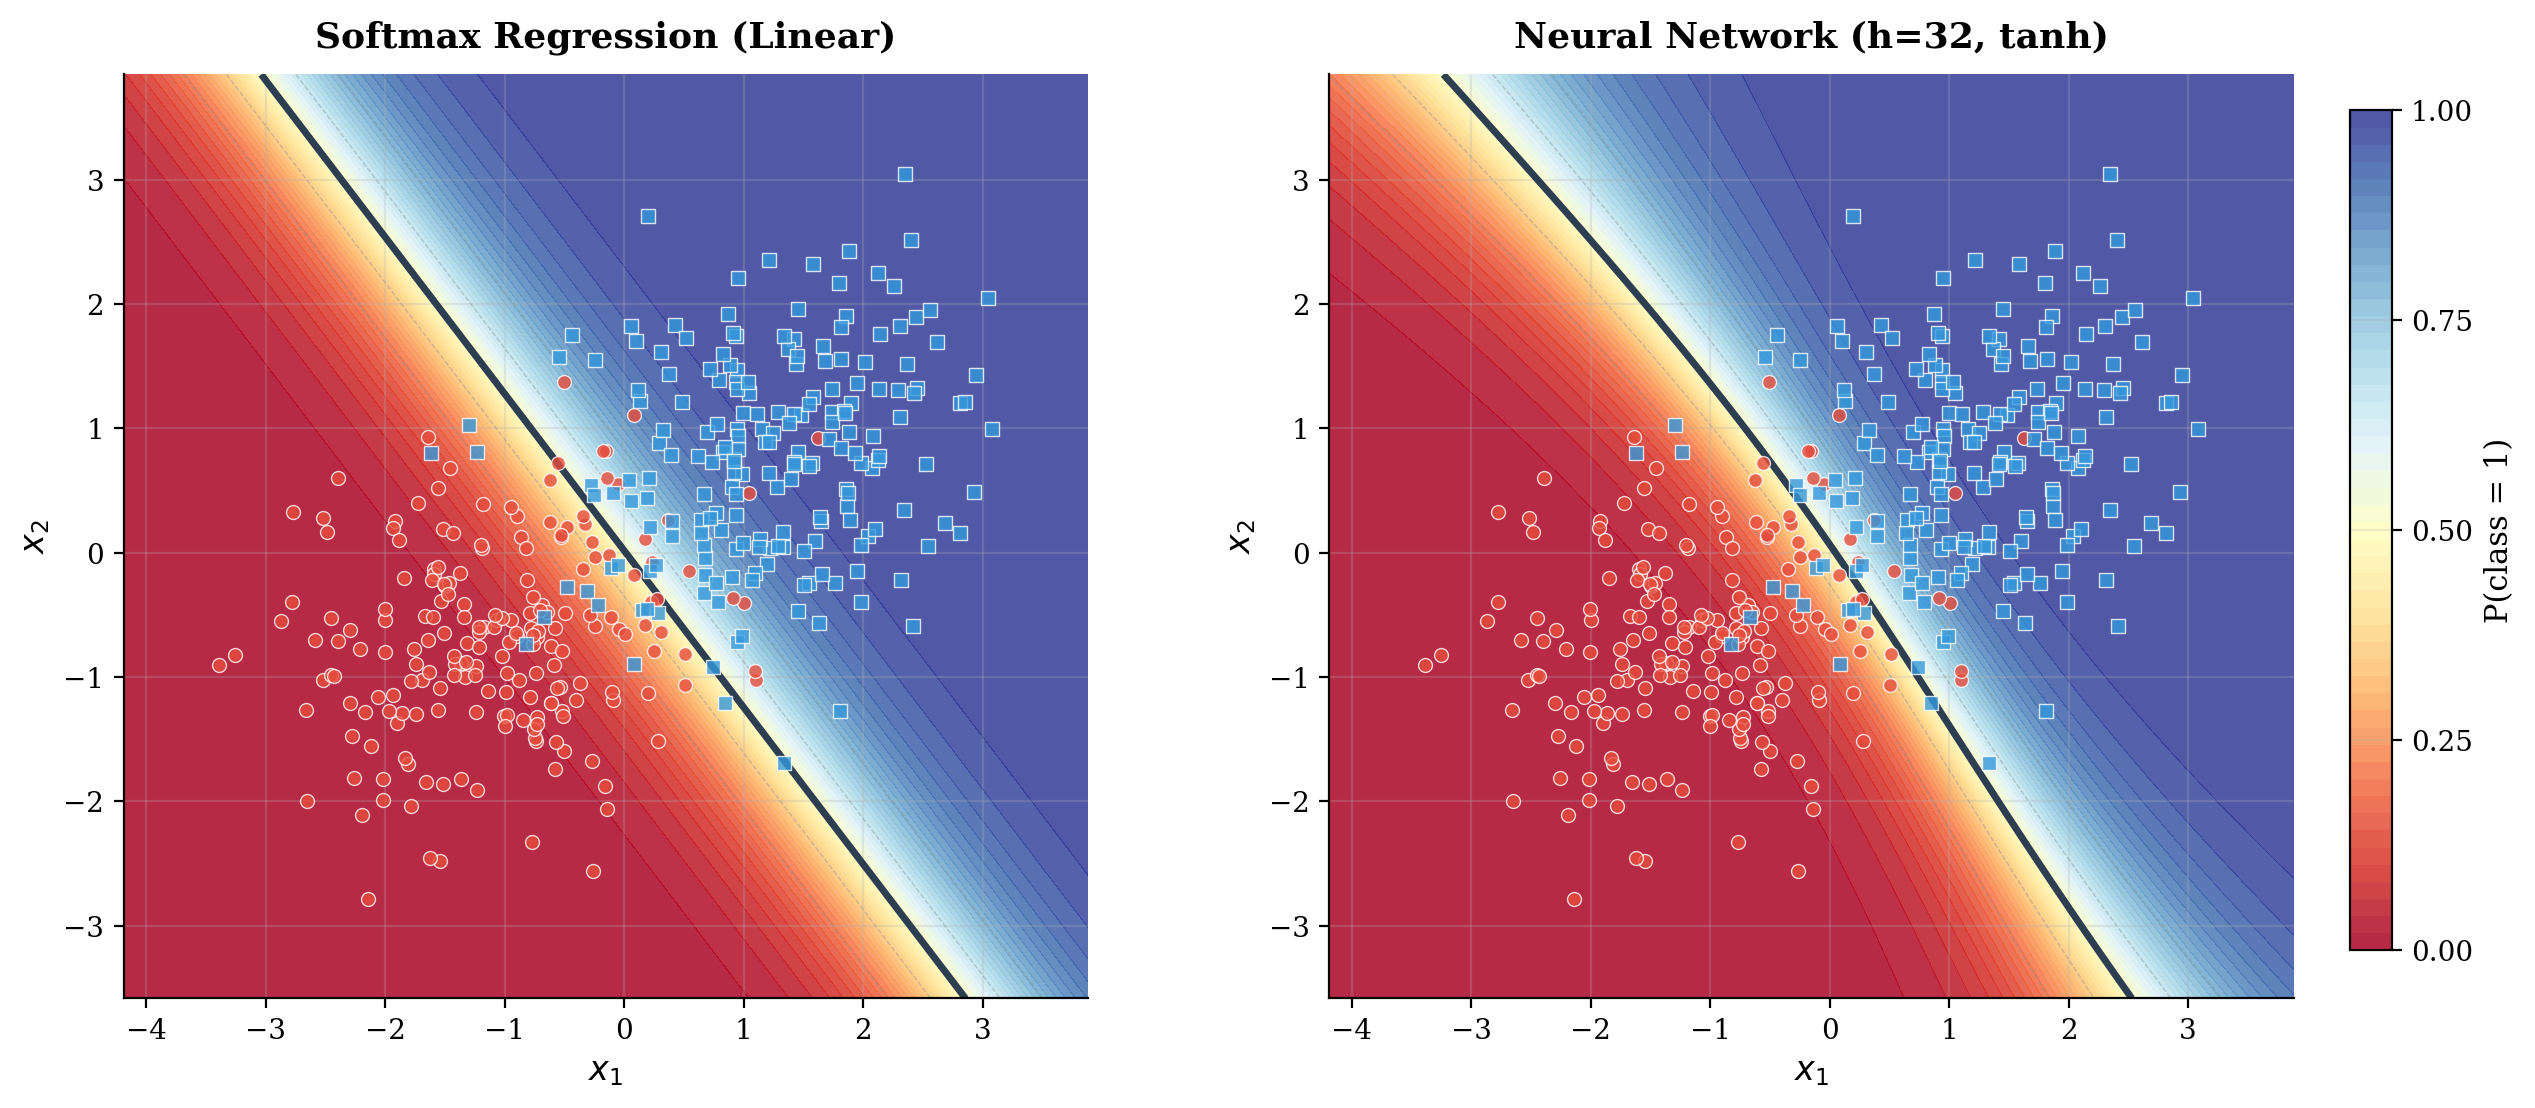
\includegraphics[width=\textwidth]{comparison_lineargaussian.png}
\end{column}
\begin{column}{0.38\textwidth}
\begin{block}{Key Finding}
Bayes-optimal boundary is a hyperplane $\Rightarrow$ \textbf{linear model suffices}.
\end{block}

\textbf{Mathematical reason:}\\[2pt]
{\small For shared covariance $\sigma^2 I$, the log-odds are \textit{affine} in $x$:}
{\small\[
\log\frac{P(y\!=\!1|x)}{P(y\!=\!0|x)} = \frac{(\mu_1-\mu_0)^\top x}{\sigma^2} + c
\]}

\begin{itemize}
    \item Both models learn the same boundary
    \item NN's extra parameters are wasted
    \item \textbf{Complexity does not justify itself here}
\end{itemize}
\end{column}
\end{columns}

\end{frame}

% ──────────────────────────────────────────
% SLIDE 6: Moons
% ──────────────────────────────────────────
\begin{frame}{Experiment 2: Moons --- Nonlinearity is Essential}

\begin{columns}[c]
\begin{column}{0.60\textwidth}
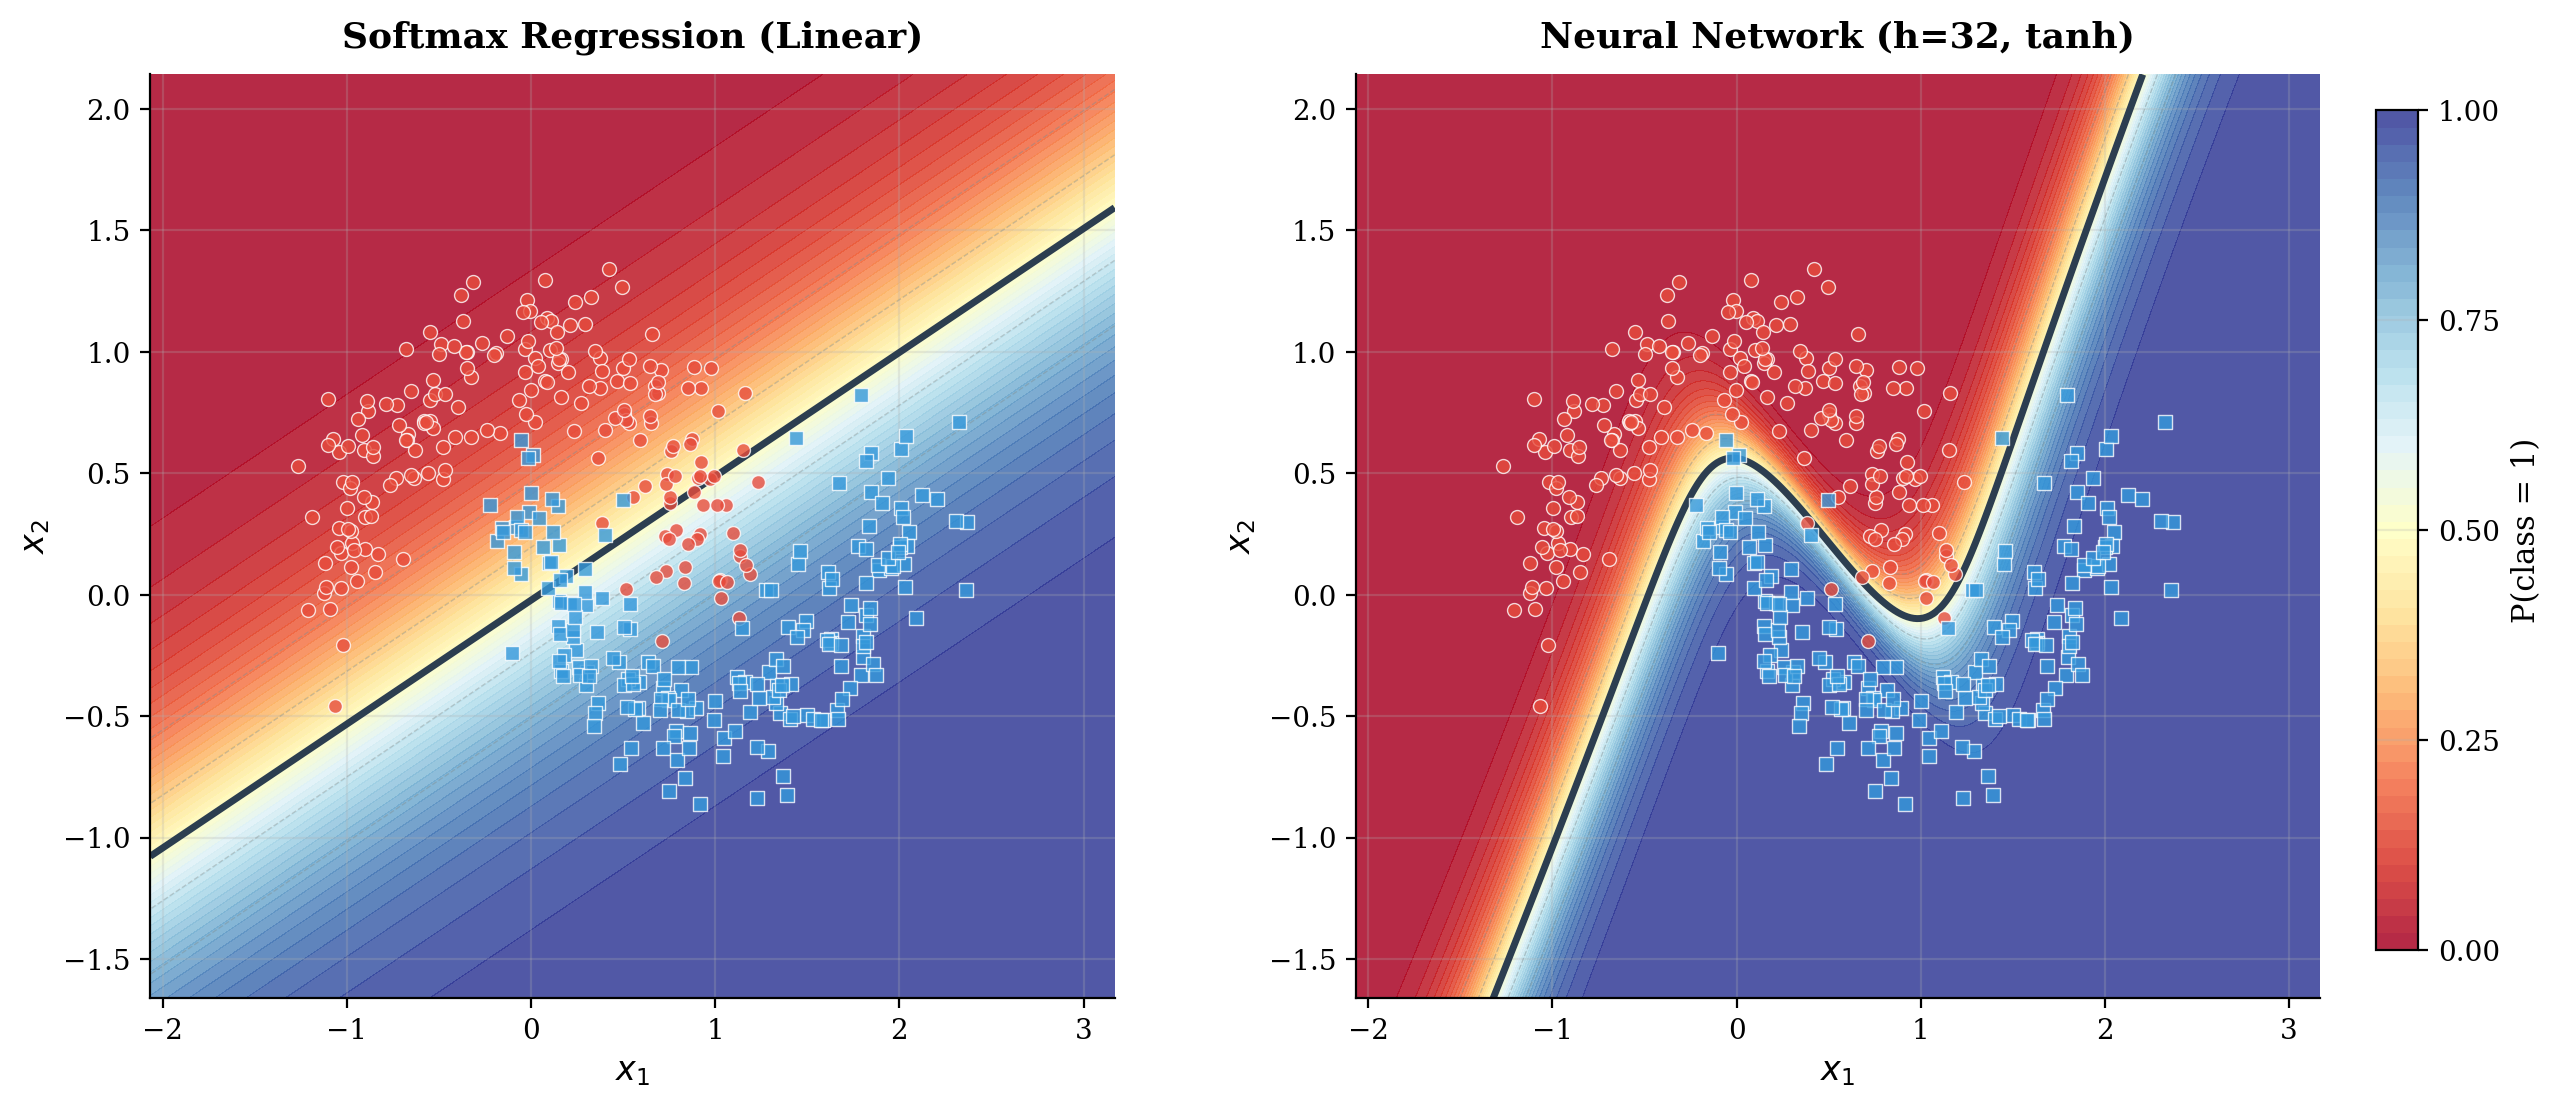
\includegraphics[width=\textwidth]{comparison_moons.png}
\end{column}
\begin{column}{0.38\textwidth}
\begin{block}{Key Finding}
Interleaving arcs are \textbf{not linearly separable} --- no hyperplane can separate them.
\end{block}
\begin{itemize}
    \item Softmax places a line through both classes $\Rightarrow$ fails
    \item NN learns a curved boundary $\Rightarrow$ near-100\% accuracy
\end{itemize}

\vspace{0.3em}
\textbf{What the hidden layer does:}\\[2pt]
{\small $h = \tanh(W_1 x + b_1)$ maps $\mathbb{R}^2 \to \mathbb{R}^{32}$.\\ In the new space, the arcs become linearly separable; the output layer draws a hyperplane there.}
\end{column}
\end{columns}

\end{frame}

% ──────────────────────────────────────────
% SLIDE 7: Digits Benchmark
% ──────────────────────────────────────────
\begin{frame}{Experiment 3: Digits Benchmark --- Real-World Task}

\begin{columns}[c]
\begin{column}{0.55\textwidth}
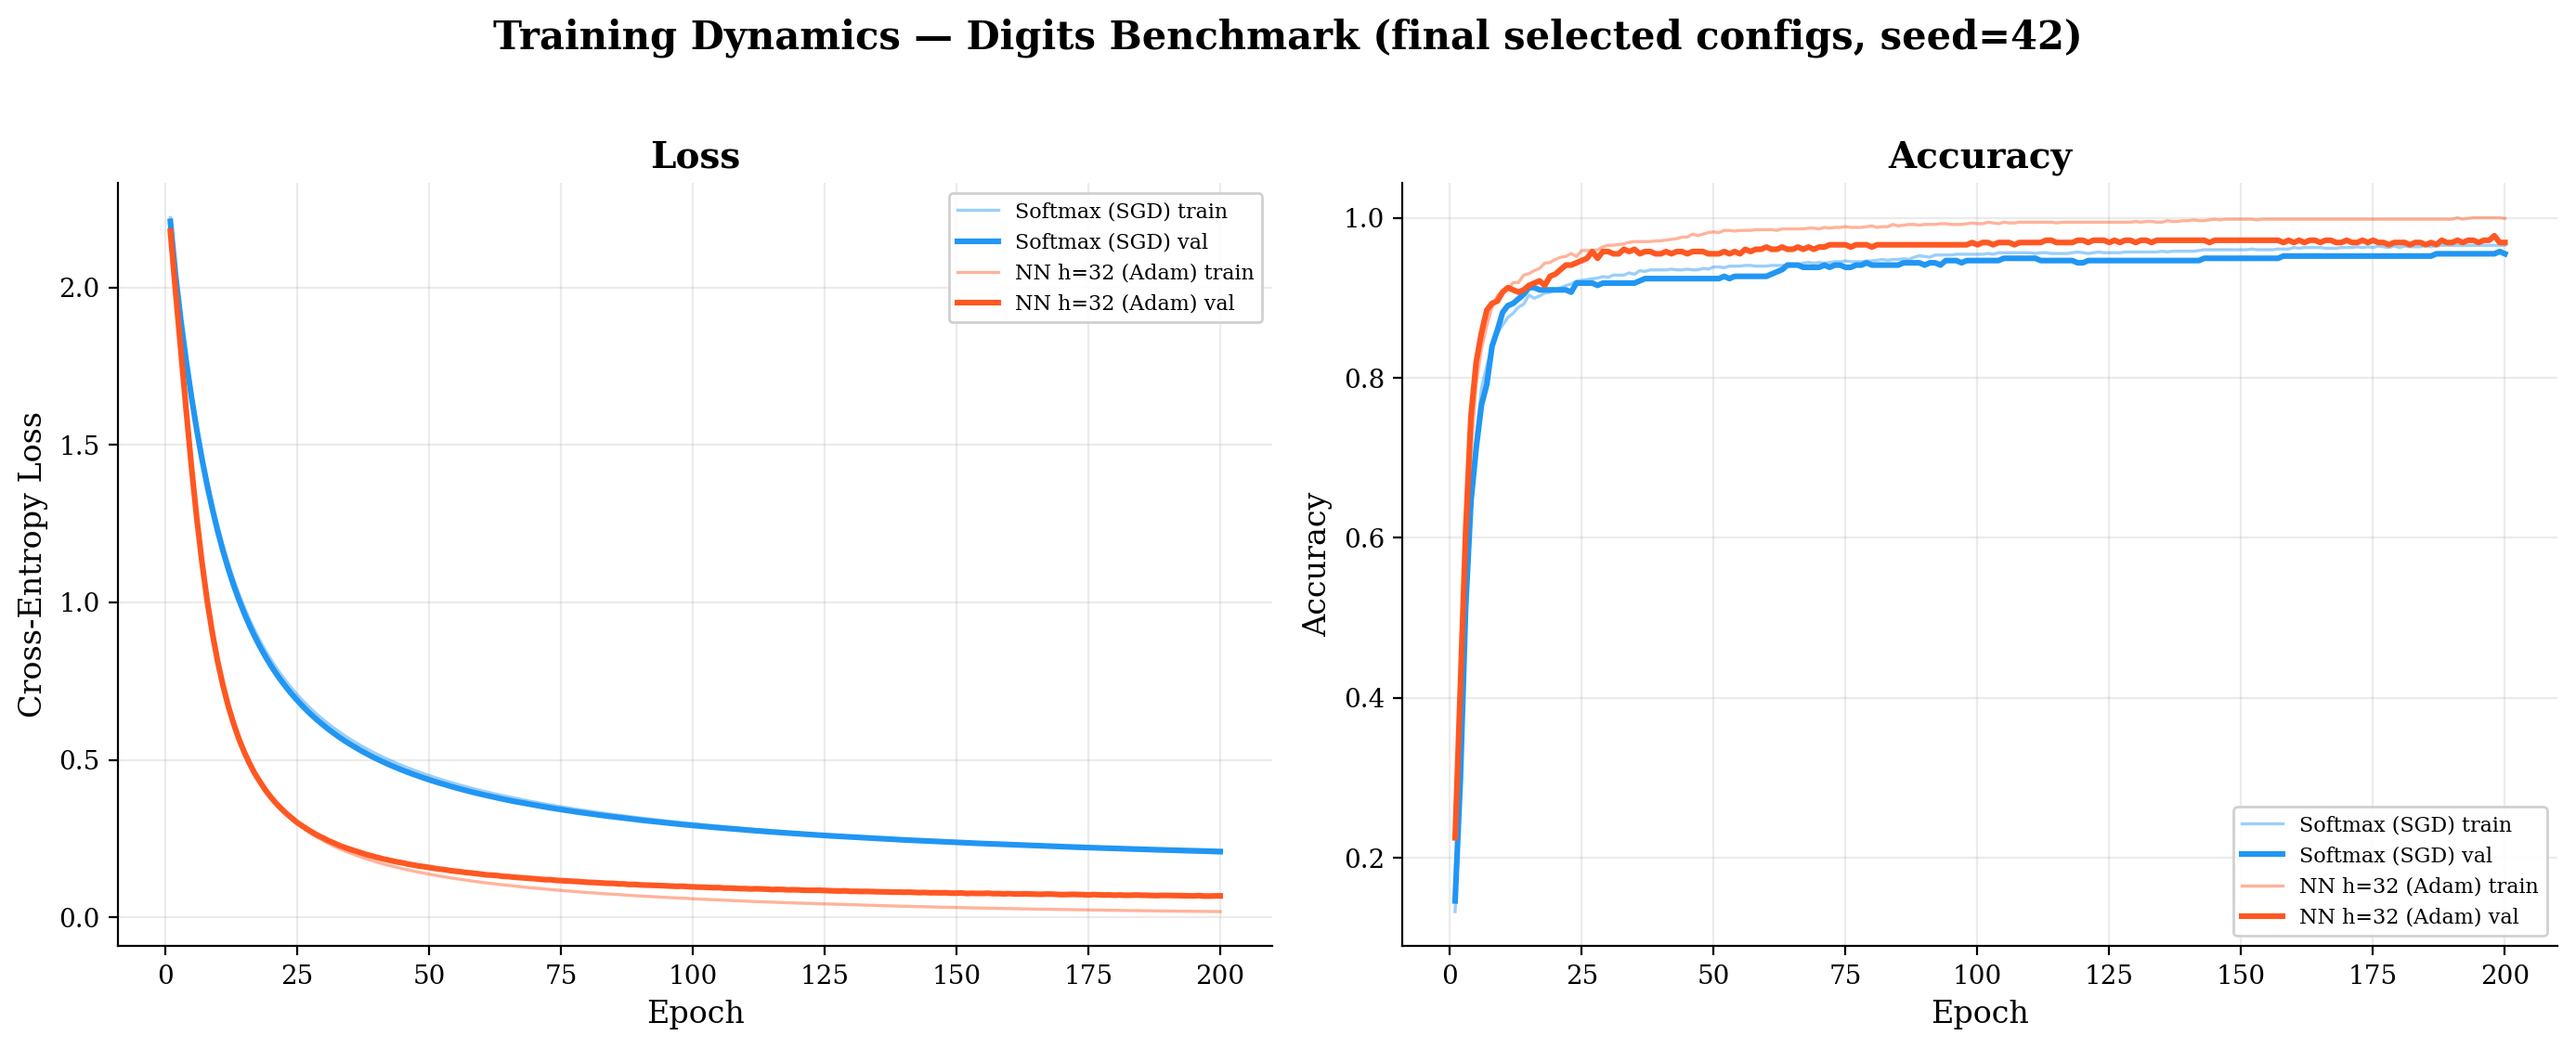
\includegraphics[width=\textwidth]{loss_curves_digits.png}
\end{column}
\begin{column}{0.43\textwidth}
\textbf{Protocol:} $d{=}64$, $K{=}10$, fixed split, $\lambda{=}10^{-4}$, batch 64, 200 epochs, best val-CE checkpoint

\vspace{0.4em}
\begin{tabular}{lcc}
\toprule
\textbf{Model} & \textbf{Acc} & \textbf{CE} \\
\midrule
Softmax & 93.3\% & 0.269 \\
NN $h\!=\!32$ & \textbf{95.7\%} & \textbf{0.157} \\
\bottomrule
\end{tabular}

\vspace{0.5em}
\begin{itemize}
    \item $\sim$2.5 ppt accuracy gain, 42\% lower CE
    \item CE reduction $>$ accuracy gain $\Rightarrow$ NN gives better-calibrated probabilities
    \item Linear model is already strong (93\%) --- Digits is ``mostly linear''
\end{itemize}
\end{column}
\end{columns}

\end{frame}

% ──────────────────────────────────────────
% SLIDE 8: Capacity Ablation
% ──────────────────────────────────────────
\begin{frame}{Capacity Ablation: Hidden Width on Moons $\{2, 8, 32\}$}

\begin{columns}[c]
\begin{column}{0.65\textwidth}
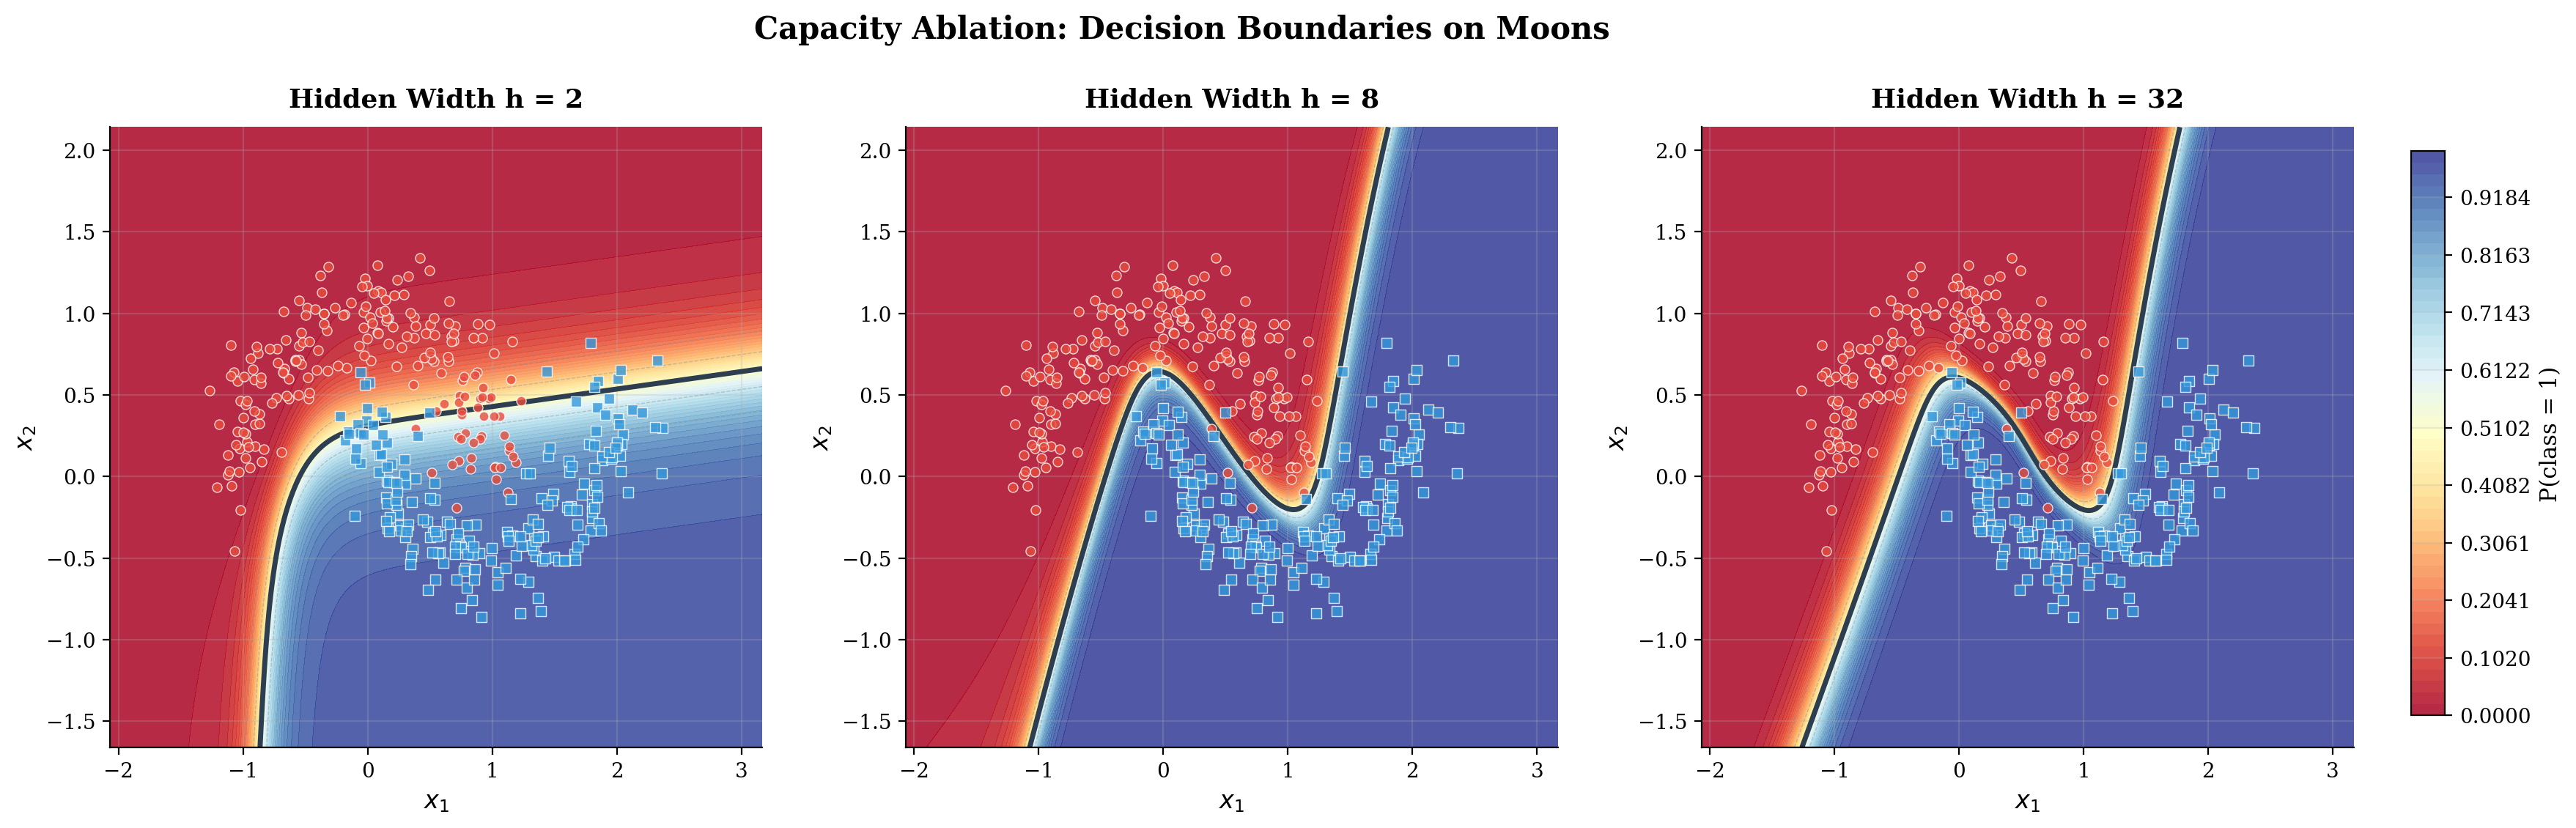
\includegraphics[width=\textwidth]{capacity_ablation_boundaries.png}
\end{column}
\begin{column}{0.33\textwidth}
\begin{itemize}
    \item \textbf{$h\!=\!2$:} crude, nearly linear separation --- too few dimensions to represent the curve
    \item \textbf{$h\!=\!8$:} smooth nonlinear boundary captures the moon shape
    \item \textbf{$h\!=\!32$:} even tighter fit, but marginal gain over $h\!=\!8$
\end{itemize}

\vspace{0.4em}
\textbf{Takeaway:} capacity must match task complexity; beyond that, returns diminish.
\end{column}
\end{columns}

\end{frame}

% ──────────────────────────────────────────
% SLIDE 9: Optimizer Study
% ──────────────────────────────────────────
\begin{frame}{Optimizer Study on Digits (NN $h\!=\!32$, fixed hyperparams)}

\begin{columns}[c]
\begin{column}{0.55\textwidth}
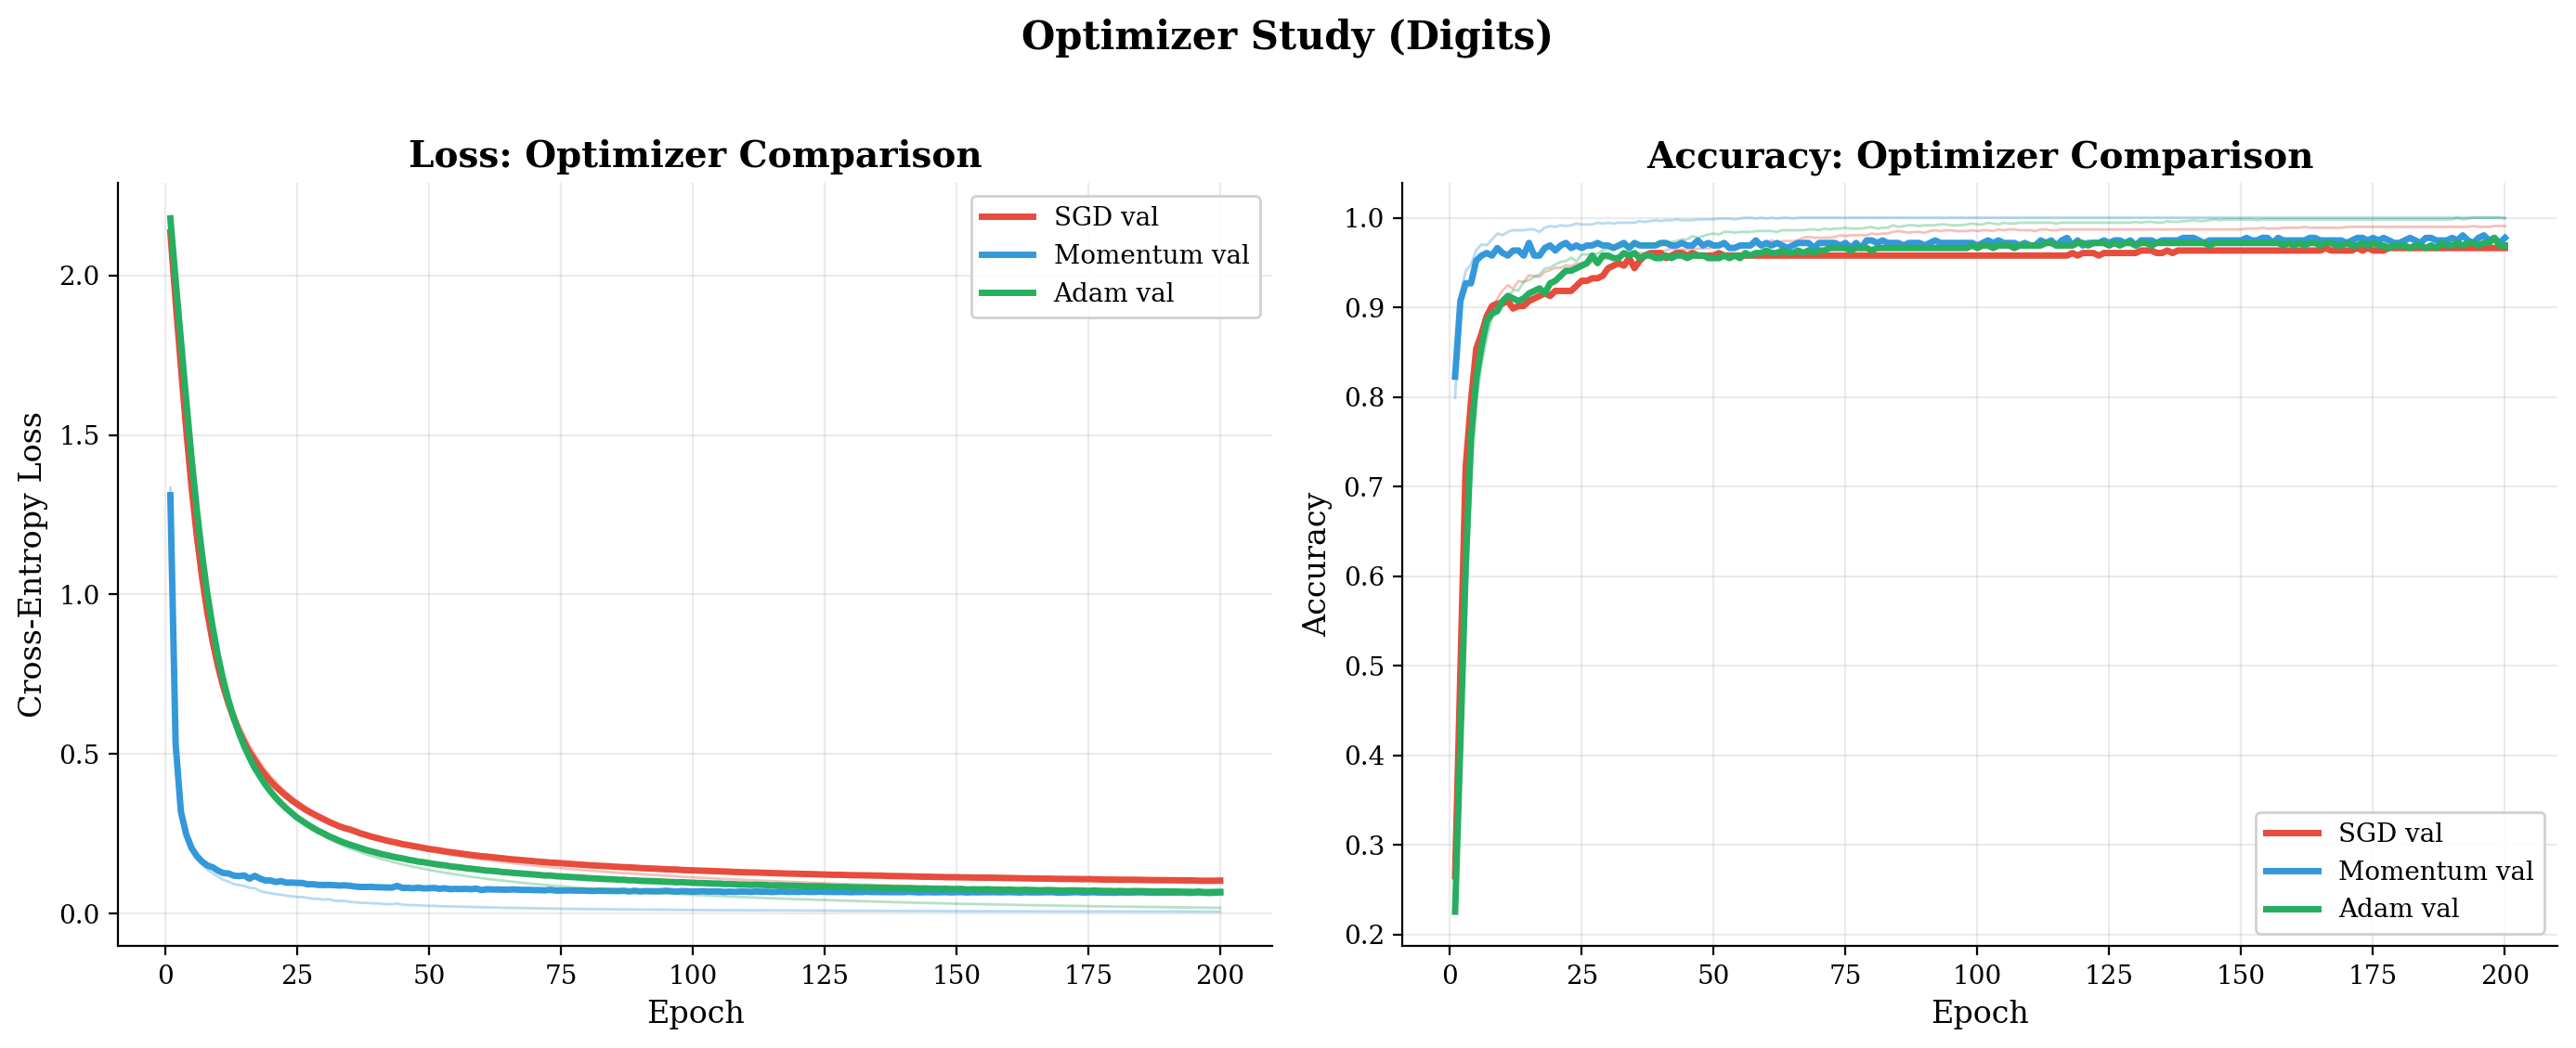
\includegraphics[width=\textwidth]{optimizer_study_digits.png}
\end{column}
\begin{column}{0.43\textwidth}

\begin{tabular}{lccc}
\toprule
\textbf{Optimizer} & \textbf{Acc} & \textbf{CE} & \textbf{Ep.} \\
\midrule
SGD & 94.8\% & 0.170 & 197 \\
Momentum & \textbf{95.4\%} & 0.165 & 197 \\
Adam & 95.1\% & \textbf{0.151} & 197 \\
\bottomrule
\end{tabular}

\vspace{0.5em}
\begin{itemize}
    \item All three reach similar final accuracy ($<$0.6 ppt spread)
    \item Adam: lowest CE (best calibration), fastest early convergence
    \item Momentum: highest accuracy
    \item \textbf{Optimizer choice is secondary to model-class choice} ($\sim$0.5 ppt vs.\ $\sim$2.5 ppt)
\end{itemize}
\end{column}
\end{columns}

\end{frame}

% ──────────────────────────────────────────
% SLIDE 10: Repeated-Seed Evaluation
% ──────────────────────────────────────────
\begin{frame}{Repeated-Seed Evaluation (5 Seeds, 95\% CI)}

\begin{columns}[c]
\begin{column}{0.45\textwidth}
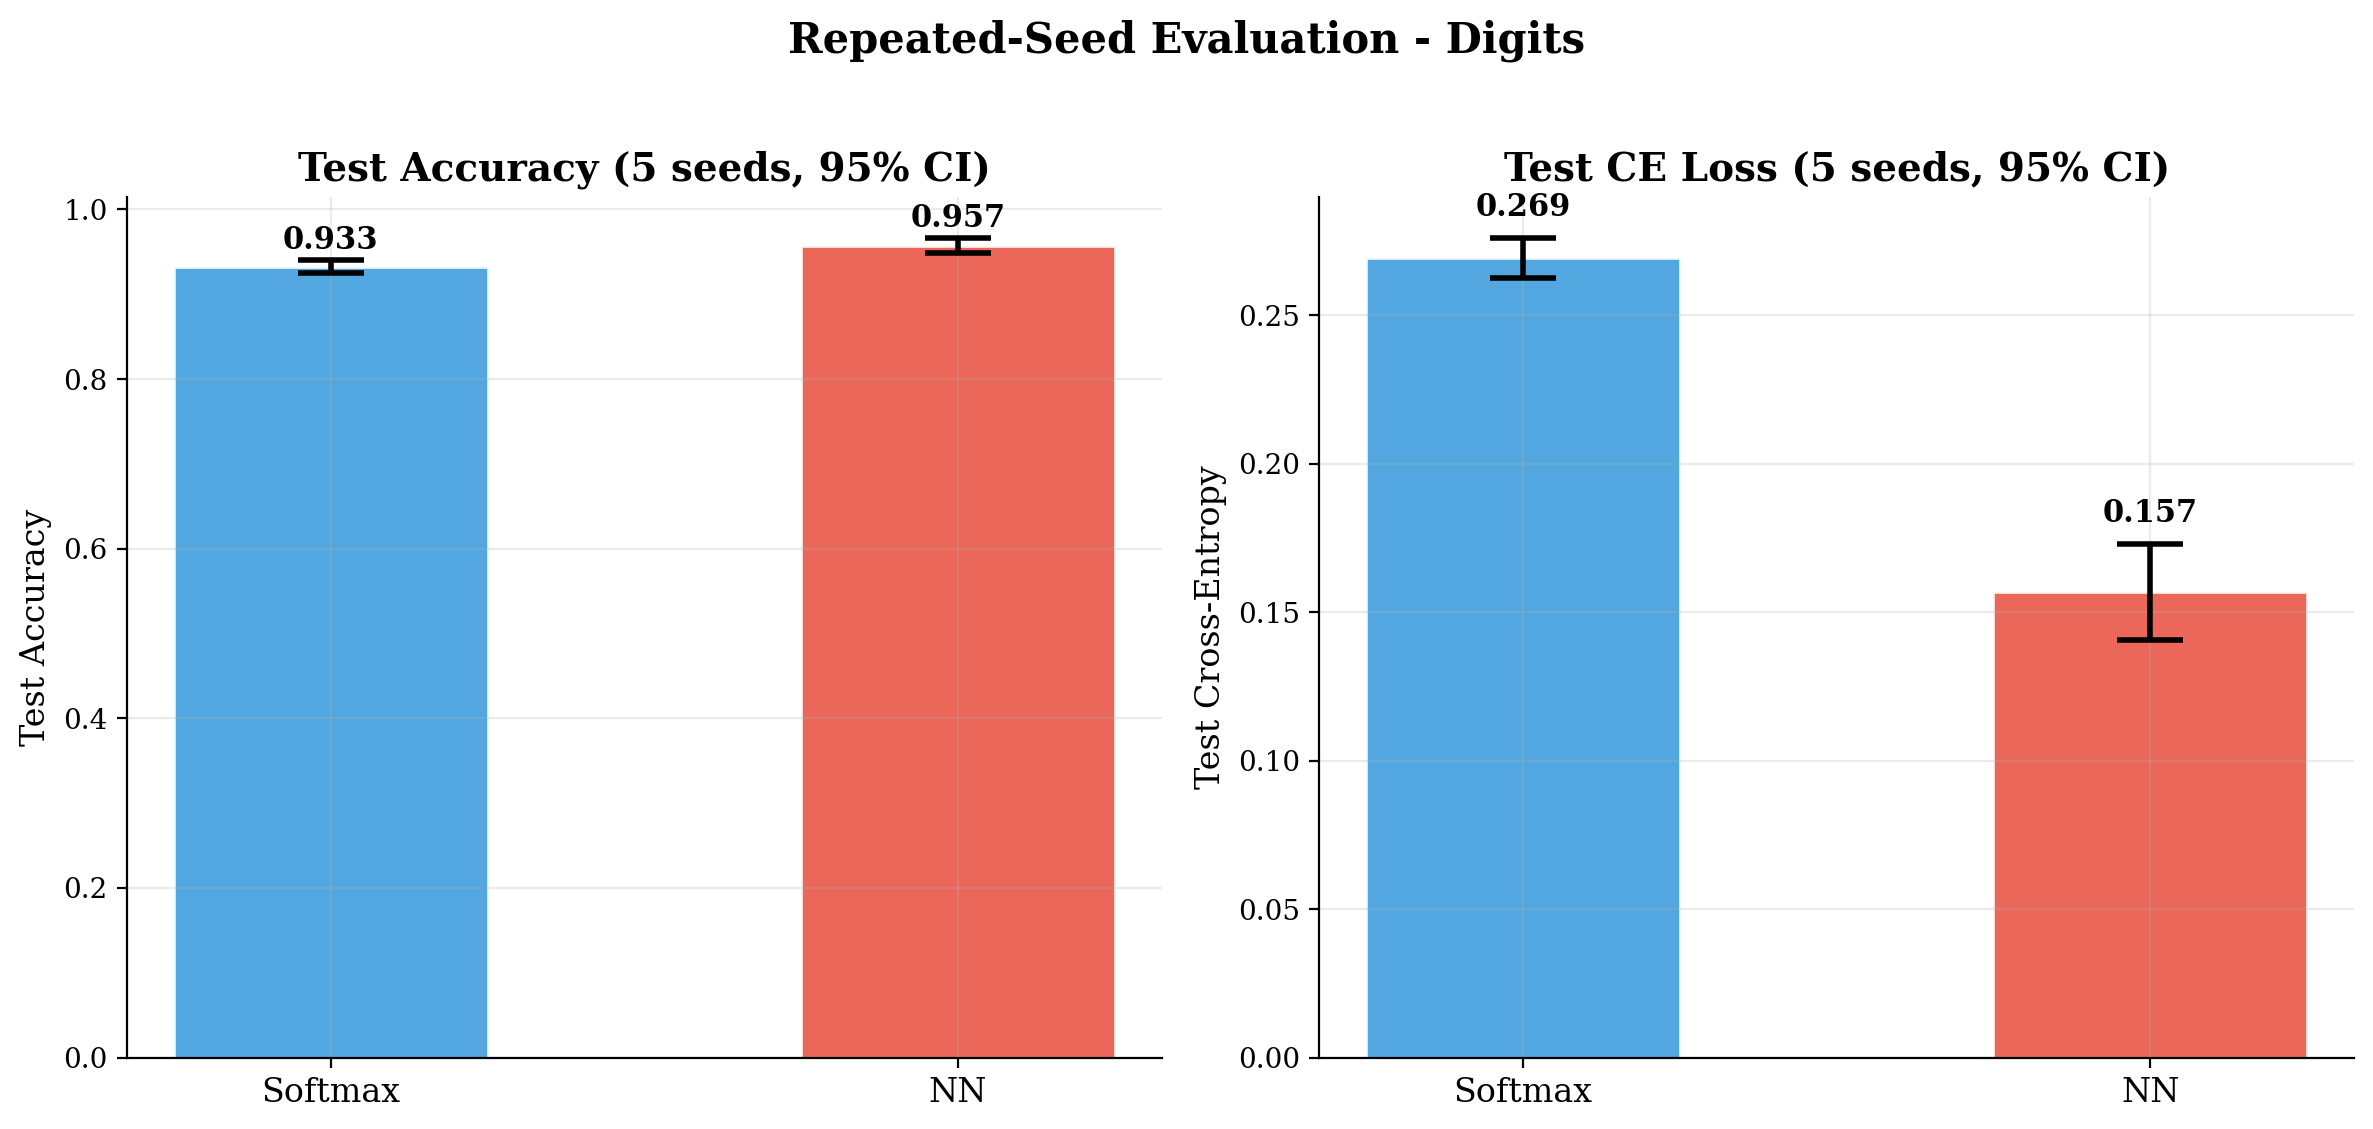
\includegraphics[width=\textwidth]{repeated_seed_digits.png}
\end{column}
\begin{column}{0.53\textwidth}
\[
\bar{x} \pm t_{0.025,\,4} \cdot \frac{s}{\sqrt{5}} = \bar{x} \pm 2.776 \cdot \frac{s}{\sqrt{5}}
\]

\vspace{0.2em}
\begin{tabular}{lcc}
\toprule
& \textbf{Test Accuracy} & \textbf{Test CE} \\
\midrule
Softmax & $93.3\% \pm 0.7\%$ & $0.269 \pm 0.007$ \\
NN & $\mathbf{95.7\% \pm 0.9\%}$ & $\mathbf{0.157 \pm 0.016}$ \\
\bottomrule
\end{tabular}

\vspace{0.4em}
\textbf{What repeated seeds add beyond a single run:}
\begin{itemize}
    \item CIs do not overlap $\Rightarrow$ NN advantage is \textbf{robust}, not a lucky seed
    \item NN has wider CI ($\pm$0.9\% vs.\ $\pm$0.7\%) --- more params $\Rightarrow$ more init sensitivity
    \item Without this, we cannot distinguish genuine model-class gains from random variation
\end{itemize}
\end{column}
\end{columns}

\end{frame}

% ──────────────────────────────────────────
% SLIDE 11: Track A - PCA/SVD
% ──────────────────────────────────────────
\begin{frame}{Track A: PCA/SVD --- How Much Linear Structure Exists?}

\begin{columns}[c]
\begin{column}{0.48\textwidth}
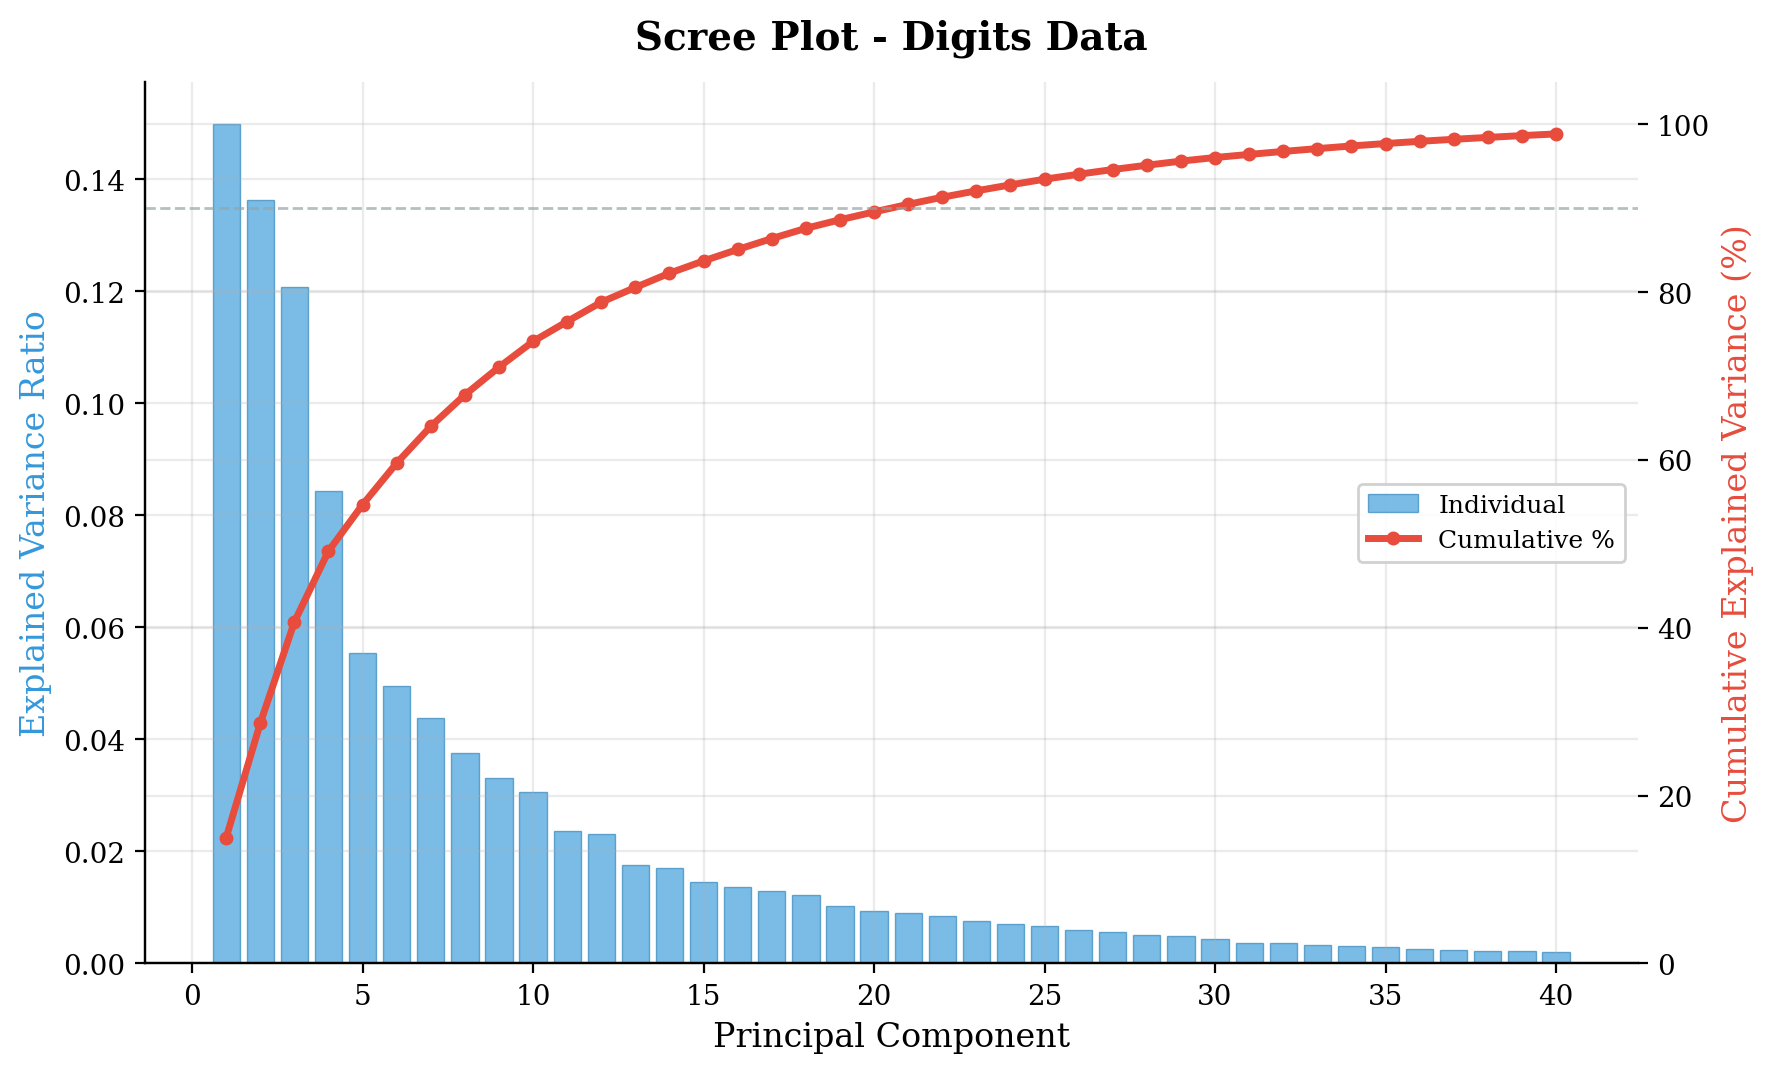
\includegraphics[width=\textwidth]{pca_scree_digits.png}

\vspace{0.2em}
\centering
\small Rapid decay: top 20 PCs capture \textbf{89.6\%} of variance
\end{column}
\begin{column}{0.48\textwidth}
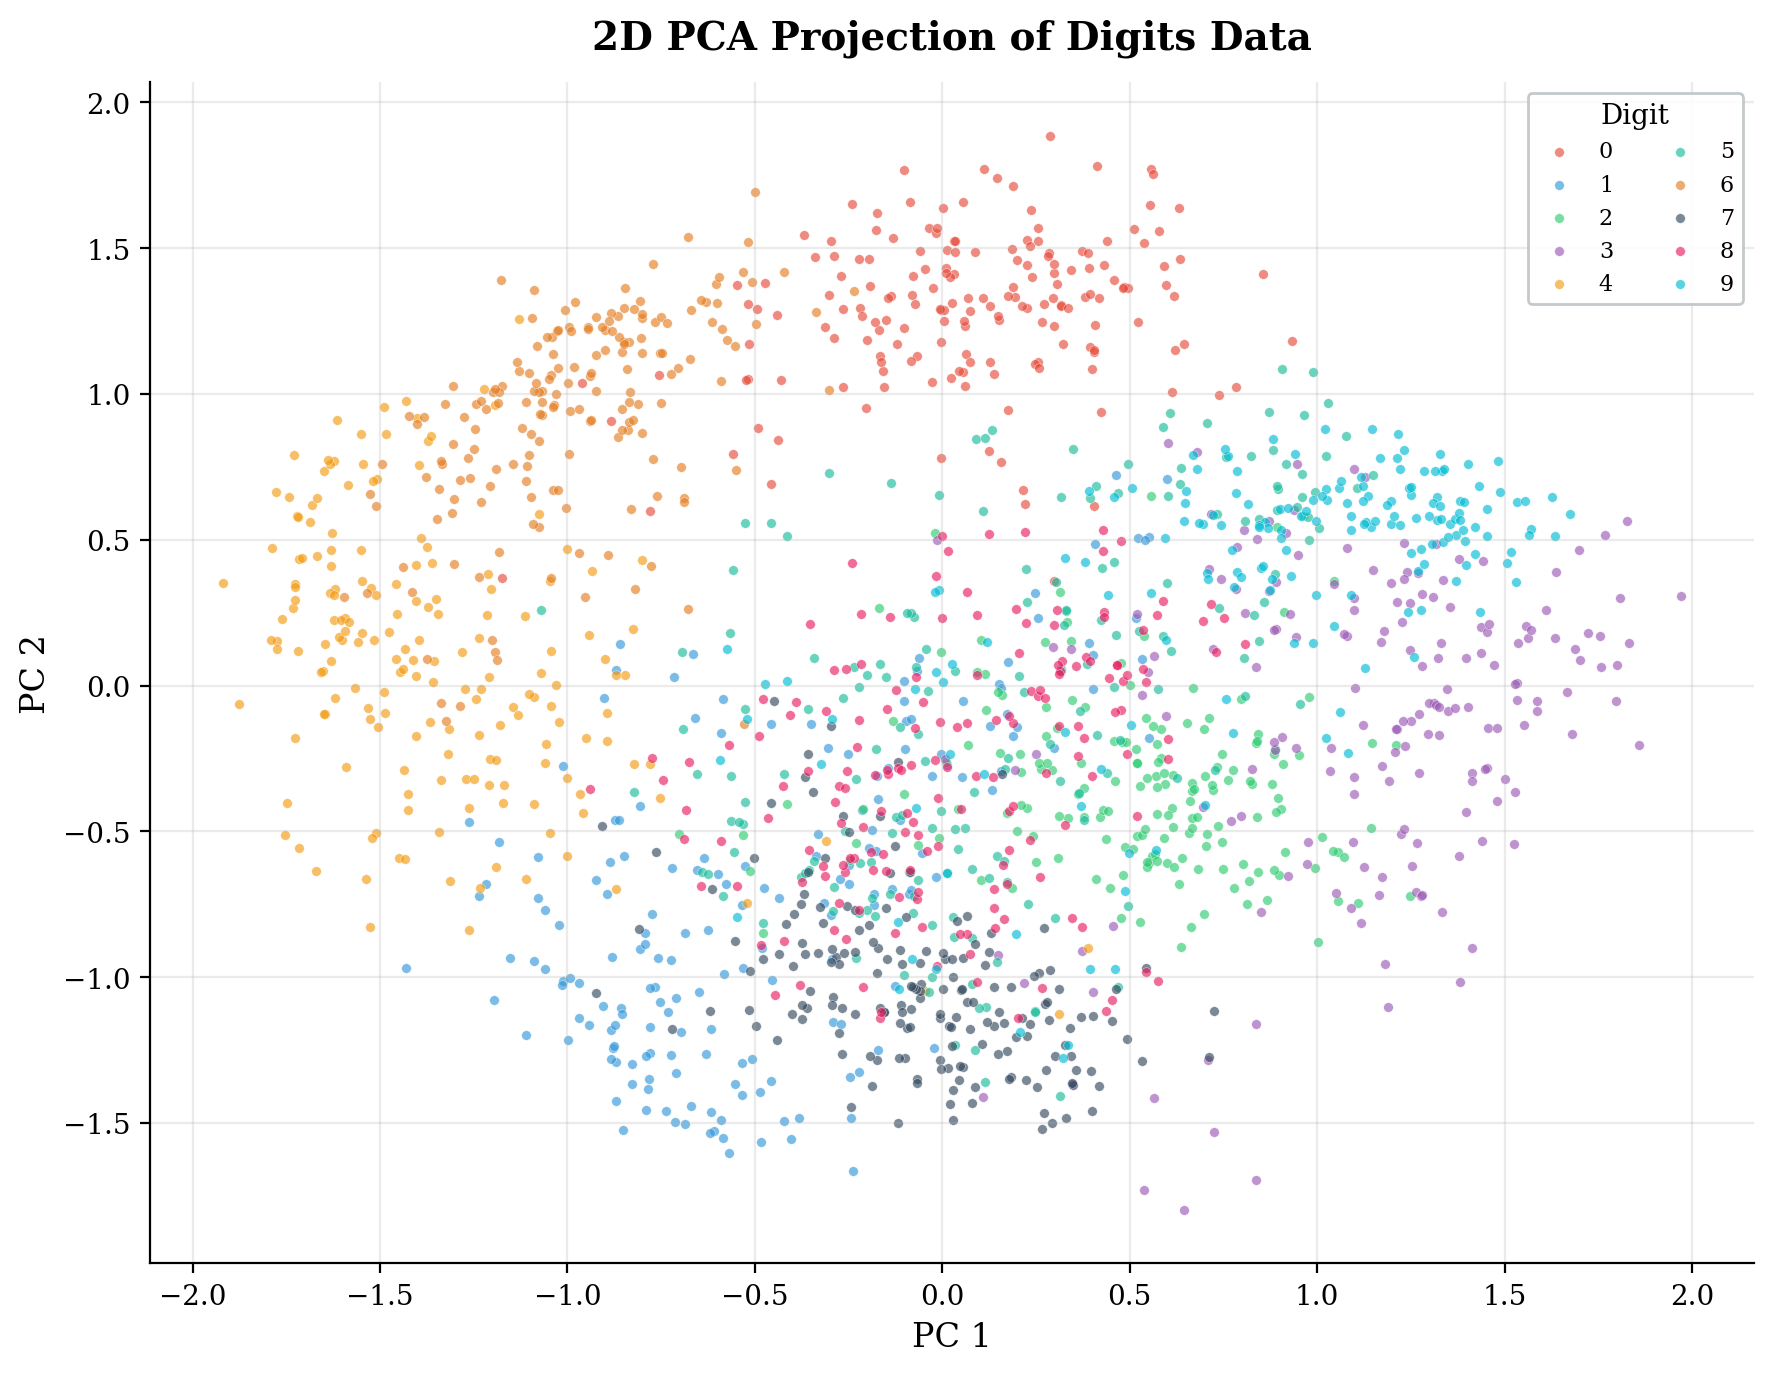
\includegraphics[width=\textwidth]{pca_2d_digits.png}

\vspace{0.2em}
\centering
\small 2D: digits 0,6 separate; 3,5,8 overlap (visual similarity)
\end{column}
\end{columns}

\vspace{0.2em}
\centering
{\small\textbf{Key insight:} The pixel space is effectively ${\sim}$20-dimensional --- most variation lives in a low-rank subspace.}

\end{frame}

% ──────────────────────────────────────────
% SLIDE 12: Track A - PCA Softmax Comparison
% ──────────────────────────────────────────
\begin{frame}{Track A: Softmax Performance vs.\ PCA Dimensions}

\begin{columns}[c]
\begin{column}{0.55\textwidth}
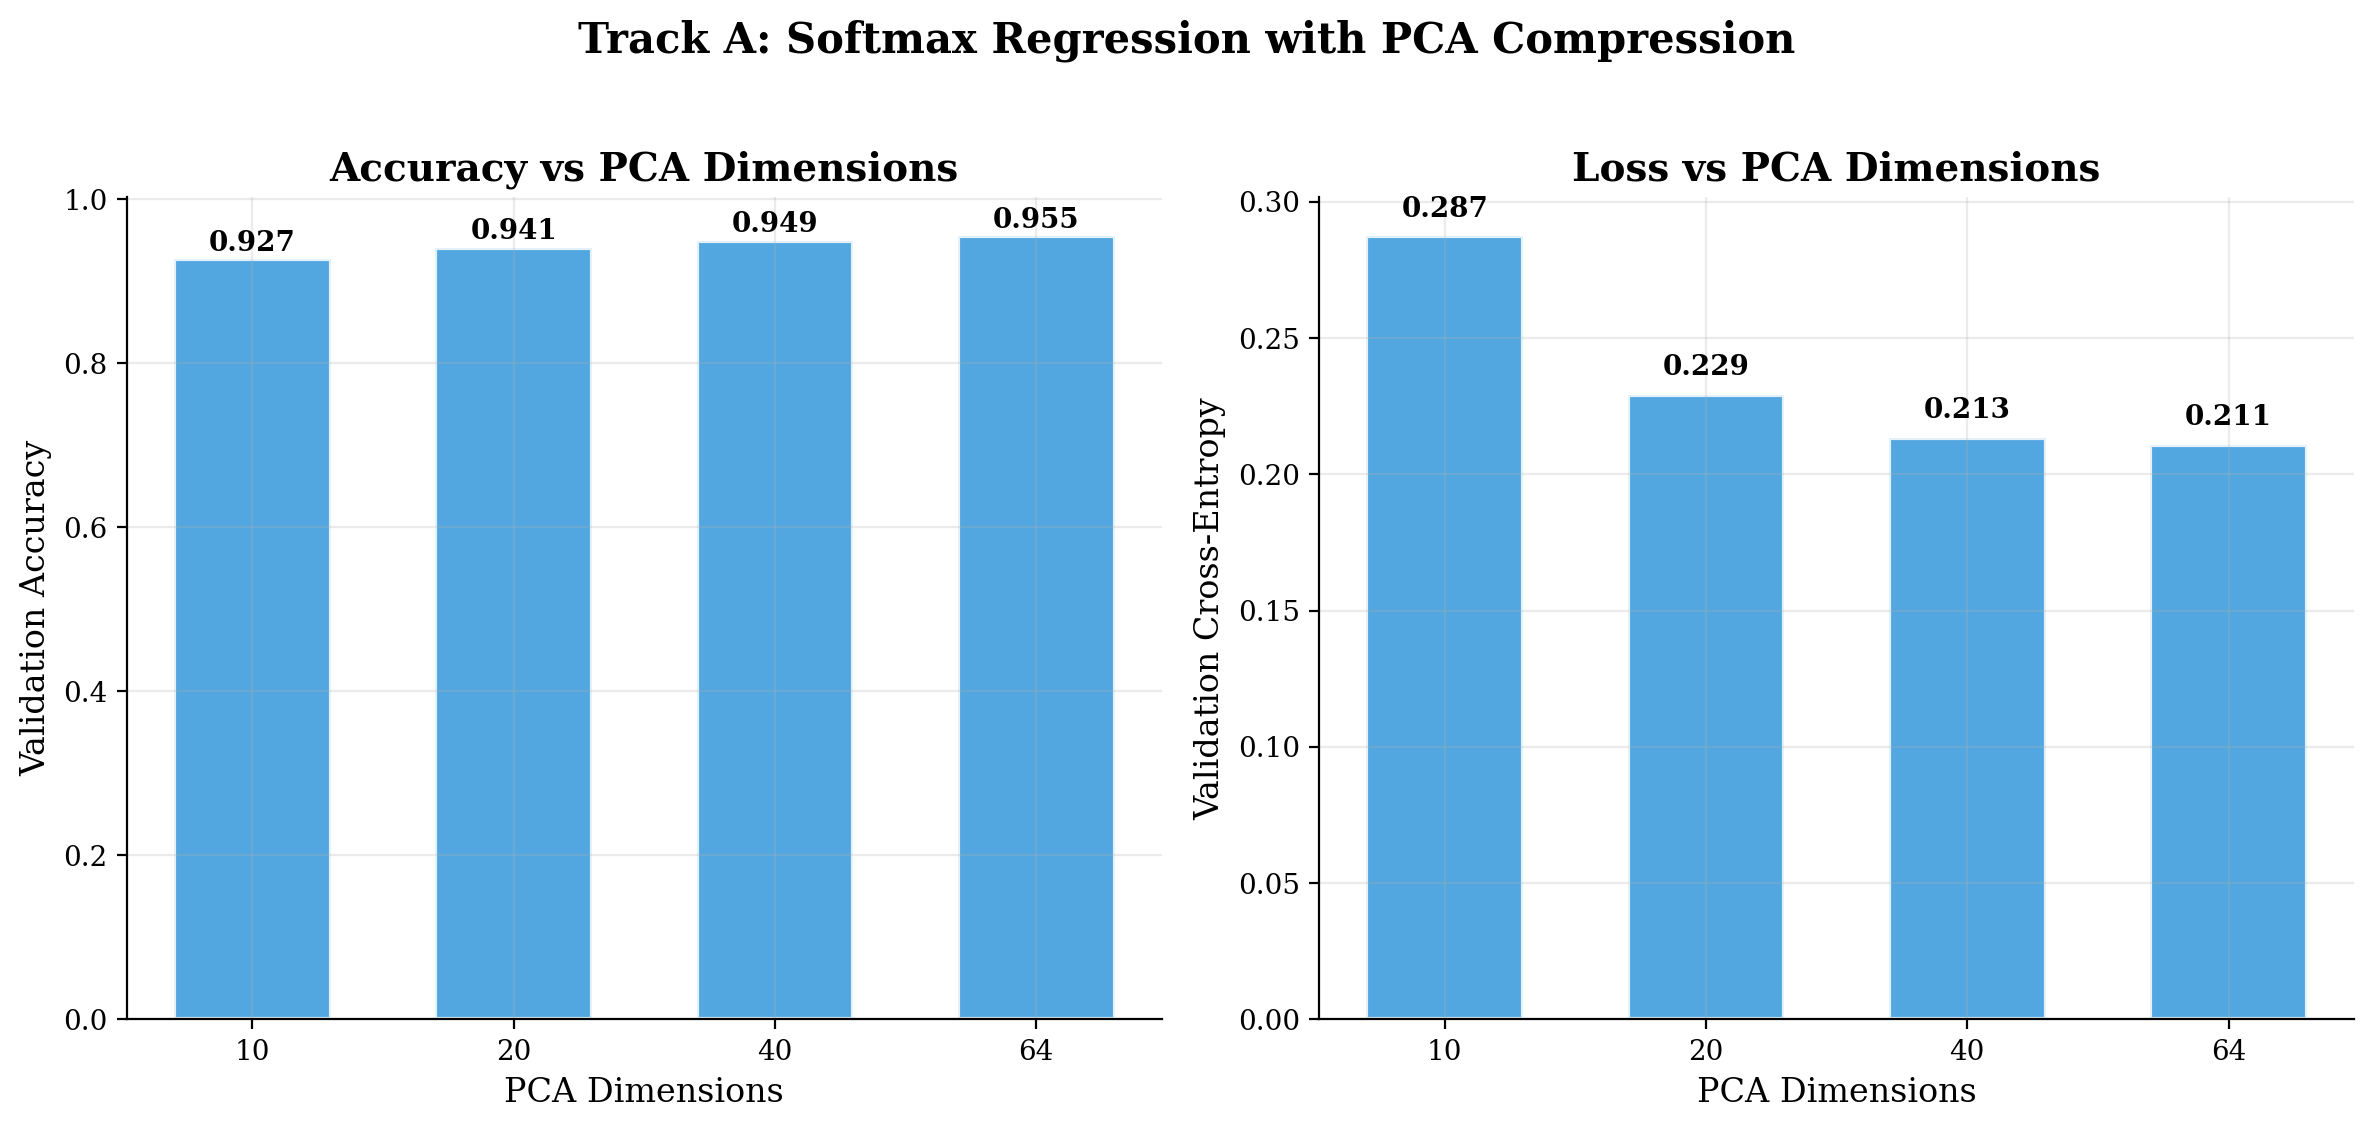
\includegraphics[width=\textwidth]{pca_softmax_comparison.png}
\end{column}
\begin{column}{0.43\textwidth}
\begin{tabular}{ccc}
\toprule
\textbf{PCA $m$} & \textbf{Val Acc} & \textbf{Val CE} \\
\midrule
10 & 92.7\% & 0.287 \\
20 & 94.1\% & 0.229 \\
40 & 94.9\% & 0.213 \\
64 (full) & 95.5\% & 0.211 \\
\bottomrule
\end{tabular}

\vspace{0.5em}
\begin{itemize}
    \item $m{=}20$: discard 69\% of dims, lose only 1.4 ppt
    \item Digits is ``mostly linear'' --- linear methods already capture most discriminative structure
    \item NN at full 64 dims (95.7\%) still beats Softmax at any PCA level $\Rightarrow$ \textbf{nonlinear features add value beyond what PCA captures}
\end{itemize}
\end{column}
\end{columns}

\end{frame}

% ──────────────────────────────────────────
% SLIDE 13: Failure Case
% ──────────────────────────────────────────
\begin{frame}{Failure Case: Under-Capacity NN ($h\!=\!2$) on 10-Class Digits}

\begin{columns}[c]
\begin{column}{0.55\textwidth}
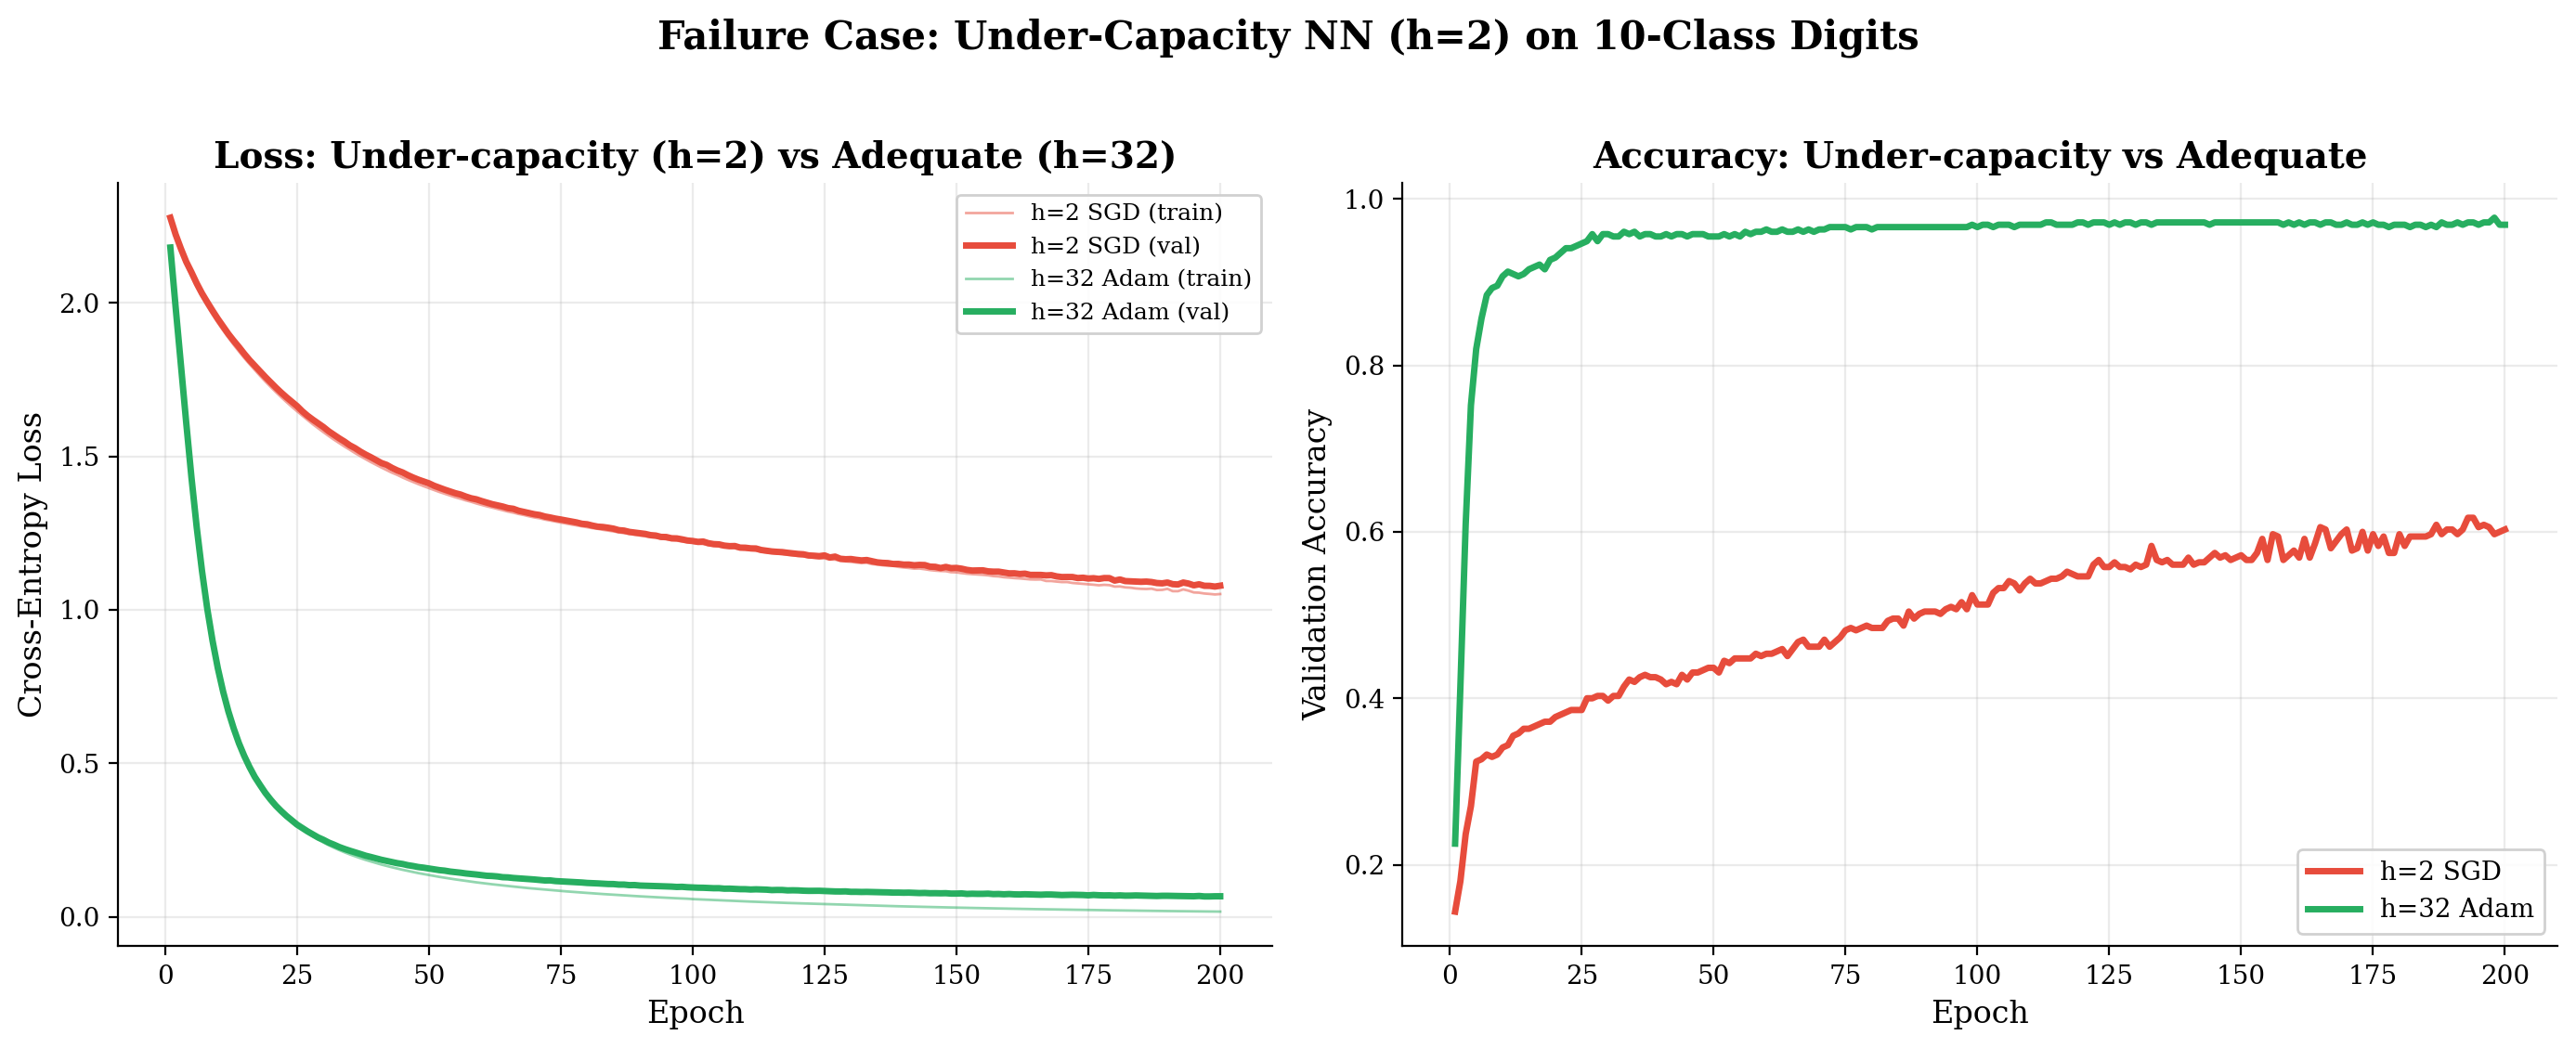
\includegraphics[width=\textwidth]{failure_analysis.png}
\end{column}
\begin{column}{0.43\textwidth}

{\small
\begin{tabular}{lcc}
\toprule
& \textbf{Acc} & \textbf{CE} \\
\midrule
Softmax (linear) & 93.3\% & 0.269 \\
NN $h\!=\!2$ & \textcolor{accentred}{59.0\%} & \textcolor{accentred}{1.113} \\
NN $h\!=\!32$ & 95.7\% & 0.157 \\
\bottomrule
\end{tabular}
}

\vspace{0.3em}
{\small\textbf{Why it fails --- capacity, not optimisation:}}
\begin{itemize}\itemsep0.1em
    \item {\small 2-D bottleneck \textbf{destroys} 64-D information}
    \item {\small Same optimizer \& epochs as $h{=}32$ $\Rightarrow$ not optimizer}
    \item {\small Train + val loss stay high $\Rightarrow$ \textbf{underfitting}}
    \item {\small \textcolor{accentred}{Worse than linear!} Hidden layer can \textit{hurt}}
\end{itemize}
\end{column}
\end{columns}

\vspace{0.1em}
\centering
{\small\textbf{Lesson:} Capacity must match task complexity \textit{before} optimisation can help.}

\end{frame}

% ──────────────────────────────────────────
% SLIDE 14: Discussion (Q1-Q2)
% ──────────────────────────────────────────
\begin{frame}{Answering the Core Questions (1/3)}

\begin{block}{\textbf{Q1:} When is the linear model geometrically sufficient?}
When the Bayes-optimal boundary is a hyperplane.  Rigorously true for Gaussian (log-odds are affine); approximately true for Digits (93.3\% linear accuracy; PCA at $m{=}20$ still gives 94.1\%).
The linear model is \textit{insufficient} when boundaries must curve (Moons).
\end{block}

\vspace{0.8em}

\begin{block}{\textbf{Q2:} What representational change does the hidden layer provide?}
$h = \tanh(W_1 x + b_1)$: a learned nonlinear coordinate change.\\
\textbf{Moons:} ``untwists'' interleaving arcs so they become linearly separable in $\mathbb{R}^{32}$.\\
\textbf{Digits:} extracts nonlinear feature combinations (stroke curvatures, junctions) that PCA cannot capture --- accounting for the $\sim$2.5-point gain.
\end{block}

\end{frame}

% ──────────────────────────────────────────
% SLIDE 14b: Discussion (Q3-Q4)
% ──────────────────────────────────────────
\begin{frame}{Answering the Core Questions (2/3)}

\begin{block}{\textbf{Q3:} When does additional complexity fail to justify itself?}
(a) When the baseline already captures the geometry (Gaussian: NN $\approx$ Softmax).\\
(b) Wrong kind of complexity ($h{=}2$ bottleneck: \textit{worse} than linear).\\
(c) Softmax at 20 PCA dims ($94.1\%$) is within 1.6 ppt of the full NN ($95.7\%$).
\end{block}

\vspace{0.8em}

\begin{block}{\textbf{Q4:} What does the failure case teach about optimisation, capacity, or generalisation?}
The $h{=}2$ bottleneck teaches that \textbf{representational capacity is a prerequisite optimisation cannot substitute}.  Same optimizer, same $\eta$, same epochs --- yet 59\% vs.\ 95.7\%.\\[3pt]
Three distinct failure modes exist:
\begin{itemize}
  \item \textit{Optimisation failure:} architecture can represent a good solution, but optimizer can't find it.
  \item \textit{Capacity failure:} architecture \textit{cannot} represent a good solution. \textbf{$\leftarrow$ this case.}
  \item \textit{Generalisation failure:} model fits training data but not test data (overfitting).
\end{itemize}
\end{block}

\end{frame}

% ──────────────────────────────────────────
% SLIDE 14c: Discussion (Q5)
% ──────────────────────────────────────────
\begin{frame}{Answering the Core Questions (3/3)}

\begin{block}{\textbf{Q5:} What do repeated-seed statistics add beyond a single run?}
A single run depends on random init and mini-batch order --- it can be ``lucky'' or ``unlucky.''\\[3pt]
Five seeds + 95\% CI show: the 2.5-point NN advantage is \textbf{robust across seeds}, not an artefact.  The NN has slightly higher variance ($\pm$0.9\% vs.\ $\pm$0.7\%), consistent with more parameters creating more initialisation sensitivity.\\[3pt]
Without this, we cannot distinguish genuine model-class gains from random variation.
\end{block}

\end{frame}

% ──────────────────────────────────────────
% SLIDE 15: Limitations
% ──────────────────────────────────────────
\begin{frame}{Limitations --- What Our Study Does Not Show}

\begin{columns}[T]
\begin{column}{0.48\textwidth}
\textbf{Scope constraints:}
\begin{itemize}
    \item Single hidden layer, $\tanh$ only --- deeper networks or ReLU may behave differently
    \item Small-scale data (${\sim}1{,}800$ samples, $d{=}64$) --- conclusions may not transfer to ImageNet-scale tasks
    \item Only $L_2$ regularisation ($\lambda{=}10^{-4}$) --- dropout, batch norm, or LR scheduling could shift results
    \item Single fixed train/val/test split --- cross-validation would be more robust
\end{itemize}
\end{column}
\begin{column}{0.48\textwidth}
\textbf{Statistical constraints:}
\begin{itemize}
    \item 5 seeds assume approximate normality --- hard to verify with $n{=}5$
    \item Each optimizer tested at one fixed setting --- not a claim about optimizer families
    \item No formal calibration analysis (reliability diagrams, ECE)
\end{itemize}

\vspace{0.5em}
\textbf{What we \textit{can} claim:}\\
Our findings reliably characterise \textit{this specific comparison} on \textit{these three tasks} under \textit{this fixed protocol}.
\end{column}
\end{columns}

\vspace{0.3em}
\centering\small\textit{These boundaries are honest --- they define what our evidence supports and what it does not.}

\end{frame}

% ──────────────────────────────────────────
% SLIDE 16: Summary
% ──────────────────────────────────────────
\begin{frame}{Summary of Key Findings}

\begin{center}
\begin{tabular}{@{}lp{5.5cm}p{5.5cm}@{}}
\toprule
\textbf{Task} & \textbf{Linear model} & \textbf{Hidden layer} \\
\midrule
Gaussian & \textcolor{accentgreen}{Sufficient} --- Bayes boundary is a hyperplane & No benefit; wasted parameters \\[4pt]
Moons & \textcolor{accentred}{Fails} --- cannot separate curved arcs & \textcolor{accentgreen}{Essential} --- learns nonlinear coordinate change \\[4pt]
Digits & \textcolor{accentgreen}{Strong} (93.3\%) --- mostly linear structure & \textcolor{accentgreen}{Modest gain} (95.7\%) --- captures residual nonlinear features \\[4pt]
Digits $h{=}2$ & 93.3\% (better!) & \textcolor{accentred}{59.0\%} --- bottleneck destroys information \\
\bottomrule
\end{tabular}
\end{center}

\vspace{0.4em}

\begin{block}{One-sentence answer}
The hidden layer helps \textbf{when and only when} the task geometry requires nonlinear boundaries \textit{and} the hidden width is sufficient to represent them.
\end{block}

\end{frame}

% ──────────────────────────────────────────
% SLIDE 17: Thank You
% ──────────────────────────────────────────
\begin{frame}{}

\vfill
\centering
{\LARGE \textbf{Thank You}}

\vspace{1em}
{\large Questions?}

\vspace{2em}
\small
All code implemented from scratch in NumPy --- no autograd, no PyTorch, no scikit-learn.\\[0.5em]
Repository: \texttt{github.com/Murad-Huseynli/math4ai\_capstone}

\vfill

\end{frame}

\end{document}
